\chapter*{Lampiran}

\section{Koefisien Proses Filter}\label{lampiran:bandpass}
\begin{table}[H]
	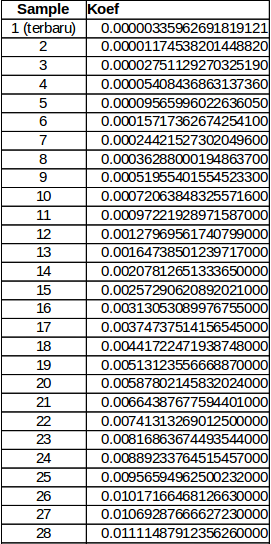
\includegraphics[scale=0.6]{images/koef1.png}
	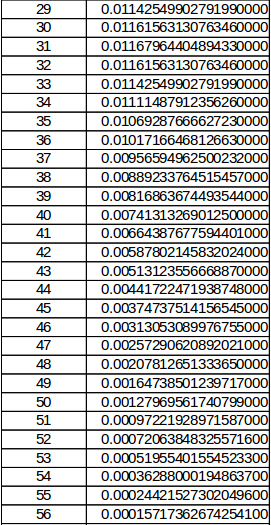
\includegraphics[scale=0.6]{images/koef2.png}
	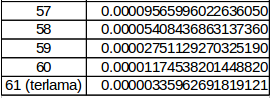
\includegraphics[scale=0.6]{images/koef3.png}
	\caption{Daftar Koefisien Band Pass Filter}
\end{table}
\begin{table}[H]
	\centering
	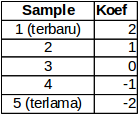
\includegraphics[scale=0.8]{images/koef4.png}
	\caption{Daftar Koefisien Derivative Filter}
\end{table}

\section{Hasil Lengkap Pengukuran Delay}\label{lampiran:delay}
\begin{table}[H]
	\centering
	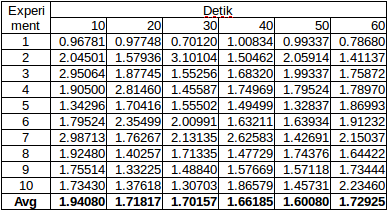
\includegraphics[scale=0.8]{images/delay_full.png}
	\caption{Delay Pada Jaringan}
\end{table}

\section{Hasil Lengkap Pengukuran Waktu Eksekusi}\label{lampiran:exec_time}
\begin{table}[H]
	\centering
	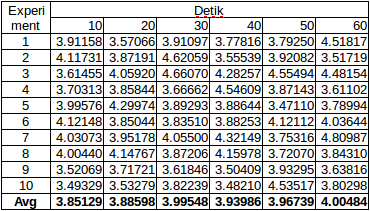
\includegraphics[scale=0.8]{images/exec_time_full1.png}
	\caption{Waktu Eksekusi DAU}
\end{table}
\begin{table}[H]
	\centering
	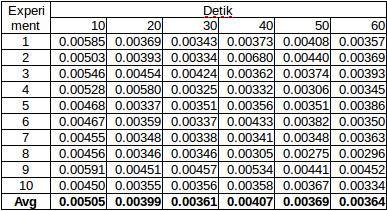
\includegraphics[scale=0.8]{images/exec_time_full2.png}
	\caption{Waktu Eksekusi SPU}
\end{table}